\documentclass[conference]{IEEEtran}
\usepackage{times}
\usepackage{amsmath,amssymb}
\usepackage{graphicx}
\usepackage{booktabs}
\setlength{\tabcolsep}{4.5pt}
\usepackage{url}
\usepackage[hidelinks]{hyperref}
\title{Detection and Recovery of UE Context\\Desynchronization in 5G RAN--Core Networks:\\A Simulation-Based Approach}
\author{
\IEEEauthorblockN{Sandesh}
\IEEEauthorblockA{\textit{Dept. of Information Technology}\\\textit{National Institute of}\\\textit{Technology Karnataka}\\Surathkal, India\\231IT061}
\and
\IEEEauthorblockN{Sujan H}
\IEEEauthorblockA{\textit{Dept. of Information Technology}\\\textit{National Institute of}\\\textit{Technology Karnataka}\\Surathkal, India\\231IT076}
\and
\IEEEauthorblockN{Laxminarayan Sahu}
\IEEEauthorblockA{\textit{Dept. of Information Technology}\\\textit{National Institute of}\\\textit{Technology Karnataka}\\Surathkal, India\\231IT035}
}
\begin{document}
\maketitle
\begin{abstract}
Fifth-generation mobile networks distribute session and resource context between the Radio Access Network (RAN) and Core. Partially completed procedures can leave these views inconsistent even when transport is reliable. This paper presents a protocol-aware verifier for a scoped, abstract RAN--Core model. The verifier compares timestamped node snapshots using semantic predicates, freshness and temporal-alignment checks, pending-procedure guards, and evidence persistence. A SimPy prototype models session establishment, QoS modification and release, and evaluates a bounded reconciliation adapter. Across 1,920 benchmark runs, the aware detector identifies all 167 QoS completion-failure episodes with zero false alarms. Under benign delay it produces no false alarms in 240 negative sessions, compared with 225 sessions for a fixed 25 ms checker. For QoS completion failures, mean detection delay is 20.93 virtual ms and mean lead time before a qualifying failed consistency probe is 18.35 ms. Recovery reduces failed probes from 334 to 148 out of 720 and total mismatch exposure from 15,698 to 6,192 session-ms. A further 720 held-out runs characterize timing sensitivity. These measurements establish behavior within the declared simulation; they do not measure actual call drops, full handover, or operator-network accuracy.
\end{abstract}
\begin{IEEEkeywords}
5G, UE context, RAN--Core consistency, protocol-aware verification, context recovery, discrete-event simulation
\end{IEEEkeywords}

\section{Introduction}
The 5G architecture distributes responsibilities among the gNB, Access and Mobility Management Function (AMF), Session Management Function (SMF), and User Plane Function (UPF). Session establishment, modification and release involve coordinated resource changes \cite{procedures,ngap}. A node can apply a requested configuration before another node completes the corresponding operation. If completion processing fails, their committed views may disagree.

This problem must be distinguished from ordinary packet loss. NGAP signaling uses reliable SCTP transport \cite{transport}. Our fault model therefore targets application request or completion handling and delayed telemetry. It does not assume that an isolated lost SCTP packet permanently removes a signaling message. N2 connects RAN and AMF control functions; N3 is the gNB--UPF user plane; N4 carries SMF--UPF control. The prototype combines Core responsibilities and does not implement an independent N4 or UPF state machine.

Aggregate monitoring can identify abnormal operational behavior, but a per-session consistency checker asks a more specific question: do the observed applied and authorized resource states satisfy a declared relationship? During valid procedures, temporary differences are expected. A detector that merely compares snapshots, or waits a fixed short time, can mistake these transitions for faults.

This project contributes an executable context model, an explainable verifier and a reproducible evaluation of bounded reconciliation. We make no claim of worldwide novelty or deployment readiness.

\section{Literature Review}
\subsection{Proposal Base Paper}
The proposal selected Cho et al.'s framework for AI-based large-scale time-series anomaly detection in 5G Core networks \cite{cho}. Its monitoring task concerns KPI streams. Point-level anomaly amplification improves sensitivity to early deviations, while distribution-aware thresholds adapt the decision rule to individual streams. This motivates timely monitoring but differs from our per-session semantic task.

Table~\ref{tab:comparison} compares scope, not reproduced performance. We do not train the cited model or claim superiority on general anomalies.
\begin{table}[t]
\caption{Comparison with the Proposal Base Paper}
\label{tab:comparison}\centering\small
\begin{tabular}{p{0.20\columnwidth}p{0.33\columnwidth}p{0.34\columnwidth}}
\toprule Aspect & Base paper \cite{cho} & This prototype\\\midrule
Input & Core KPI time series & Node-state snapshots\\
Decision & Statistical anomaly & Semantic contradiction\\
Granularity & KPI stream & UE/session pair\\
Evaluation & Operator-network study & Synthetic controlled faults\\
Recovery & Not reproduced here & Custom reconciliation\\\bottomrule
\end{tabular}
\end{table}
\subsection{Consistency and Protocol References}
Sid-Otmane et al. discuss data consistency in the 5G specification \cite{consistency}. This provides additional context for treating distributed UE state as a correctness problem. Our implementation is not a replication of that paper. 3GPP TS 23.502 and TS 38.413 provide procedure background \cite{procedures,ngap}; TS 38.300 provides access and mobility context \cite{ran}. The prototype abstracts these references rather than implementing all normative transitions.

\section{System Model and Methodology}
\subsection{Scope and State Representation}
For each key $k=(\mathrm{UE},\mathrm{session})$, the simulator stores independent RAN and Core records
\begin{equation}
C_x=(s_x,a_x,q_x,r_x,c_x,p_x,\tau_x,d_x,v_x,t_x),
\end{equation}
where $s$ denotes logical session existence, $a$ access resources, $q$ an abstract QoS profile identifier, $r$ access state, $c$ local cell, $p$ pending operation, $\tau$ transaction identity, $d$ deadline, $v$ version, and $t$ last-change time. QoS integers are not QFI or 5QI encodings.

The model is a timed extended finite-state machine (EFSM). The RAN resource control has ABSENT and APPLIED($q$) states. Core procedure control has STABLE, SETUP\_PENDING, MODIFY\_PENDING and RELEASE\_PENDING states. The committed Core record remains unchanged during a pending operation. Transaction identifiers and timestamps augment the finite control.

Both records initially have no session or resources and QoS zero. RRC begins CONNECTED because radio attachment precedes the modeled session workflow. The access controls exercise CONNECTED and IDLE; RRC\_INACTIVE is not implemented. A logical session can persist while access resources are inactive. A local cell change is a negative control, not a full handover procedure.

\subsection{Transition Relation}
The Core begins an operation by allocating a transaction and deadline. Setup targets $(s,a,q)=(1,1,1)$; modification requires a committed session and targets $(1,1,q_C+1)$; release targets $(0,0,0)$. The RAN applies a current request, and the Core commits its target only after processing a current completion. At timeout, the Core clears pending state and retains its previous committed record. The RAN retains any configuration already applied. Table~\ref{tab:transitions} specifies the principal transitions.

\begin{table}[t]
\caption{Transition Effects in the Implemented EFSM}
\label{tab:transitions}\centering\small
\begin{tabular}{p{0.25\columnwidth}p{0.27\columnwidth}p{0.35\columnwidth}}
\toprule Event & RAN effect & Core effect\\\midrule
Begin operation & Unchanged & Set pending, transaction, deadline\\
Apply current request & Apply target & Retain old record\\
Process completion & Retain target & Commit target; clear pending\\
Timeout & Retain applied state & Retain old record; clear pending\\
Stale message & Reject stale request & Reject stale completion\\
Idle/resume & Toggle access resources & Retain logical session\\
Recovery & Copy authorization & Retain committed record\\\bottomrule
\end{tabular}
\end{table}

Each session has at most one pending operation. Commit and timeout semantics are experimental choices, not mandatory 3GPP rollback behavior.

\subsection{Coupling Invariants}
The verifier evaluates three predicates:
\begin{align}
I_1 &= a_R \land \neg s_C,\\
I_2 &= (a_R \ne a_C) \land \neg I_1,\\
I_3 &= a_R \land a_C \land (q_R \ne q_C).
\end{align}
$I_1$ denotes an orphan RAN resource; $I_2$ an access-resource mismatch; and $I_3$ a QoS-profile mismatch. The orphan predicate takes precedence over a resource mismatch. Both predicates can be absent when access is inactive and the Core retains a logical session. Local cell equality is not an invariant. Absence of these predicates means consistency only with respect to these modeled relationships.

\subsection{Observation-Based Verification}
The detector receives complete snapshots containing the key, side, node sequence number, capture timestamp and context record. It never receives injected-fault flags or oracle labels. Each new snapshot replaces the previous view only if its sequence number is greater.

The aware mode applies the following guards. Both sides must be present and no more than 60 ms old. Their stable intervals must overlap:
\begin{equation}
\min(t^{cap}_R,t^{cap}_C)\geq\max(t^{chg}_R,t^{chg}_C).
\end{equation}
A pending Core operation suppresses evidence before its deadline. If a pending view remains after the deadline, a Core snapshot captured at or after that deadline is required. Accepted contradictory evidence must then persist for a default 12 ms. The monitor emits one alarm per active session/rule candidate and records both contexts and timing evidence.

Stale or incompatible observations reset evidence. They represent unknown state, not a proof of consistency. The common simulator clock is an explicit assumption. With unbounded delay and no additional observations, timeout alone cannot establish permanent message loss. Our detector relies on the modeled committed-state semantics and telemetry guarantees.

\subsection{Recovery Adapter}
On an alarm, a custom adapter queries both nodes, refuses a pending operation, and checks versions before writing. It reconciles the RAN session, resource and QoS fields to the committed Core authorization, then queries again to verify convergence. Query and actuation delays each range from 5 to 10 ms, followed by a 3 ms verification delay. A job makes at most two attempts.

Core authority is a modeling choice for these fields. This adapter is not a standardized ``Context Sync Request.'' Successful convergence may remove orphan resources and leave a UE without a usable session. State consistency and service availability are separate outcomes.

\section{Implementation and Experimental Setup}
\subsection{Software and Scenario Design}
The prototype uses Python and SimPy for virtual-time scheduling, with a Streamlit demonstration interface \cite{simpy,streamlit}. Separate modules implement the context model, simulator, verifier, metrics, command-line experiments and plots. The dashboard displays events, state views and downloadable results.

The twelve scenarios are clean operation, benign delay, request-processing failure, QoS/setup/release completion-processing failure, reordered observations, queued high load, observation outage, access idle/resume, local cell change, and unavailable recovery. Request-processing failure can prevent service without creating a contradiction; injection is therefore not itself a positive ground-truth label.

Each run contains three UEs with two sessions each over 540 virtual ms. Default monitor/oracle ticks are 2 ms, polling is 15 ms, and the procedure timeout is 110 ms. Ordinary application-leg delay is uniform over 3--9 ms; benign-delay legs use 18--42 ms. High load adds a shared three-worker processing queue with 18--42 ms service times. Fault eligibility is sampled per session with probability 0.7. This is not an independently sampled per-packet loss rate.

The main suite uses 40 seeds and four configurations: immediate checking, a fixed 25 ms mismatch checker, aware checking without recovery, and aware checking with recovery. This yields $12\times40\times4=1,920$ runs. Independent observation and recovery random-number streams preserve paired node trajectories until intervention. Additional held-out experiments use seeds 101--120, three scenarios, four polling intervals and three grace values, yielding 720 runs.

\subsection{Ground Truth and Metrics}
An oracle reads actual node states at each tick and opens a contradiction episode only after pending procedures end. The verifier consumes observations alone. Both use the same semantic predicates, so this evaluates monitoring under the declared model, not independent conformance of those predicates to the full standards.

An alarm is a true positive only if its key and rule match a truth episode and its time lies within that episode. Early alarms during valid transitions are false positives even if a contradiction develops later. Repeat alarms within an already matched episode count separately as duplicates. Precision is $TP/(TP+FP)$ and recall is detected episodes divided by all truth episodes. The false-positive rate divides negative sessions receiving a false alarm by all sessions with no truth episode in that run. Undefined denominators remain N/A; aggregation pools counts.

Detection delay starts at the oracle's episode onset. Fixed probes at 285, 335 and 510 ms fail when the actual context has a stable contradiction. Lead time is the interval from an alarm to the first subsequent failed probe in the same episode. Probes are independent of alarm timing and measure context consistency, not calls or packet delivery. Total mismatch exposure is the sum of episode durations in session-ms. Recovery success counts verified successful jobs divided by all recovery jobs.

\section{Results and Discussion}
\subsection{Detection Accuracy and Timing}
Table~\ref{tab:detection} gives aware results with recovery disabled. All listed truth episodes were detected without false alarms in these selected synthetic cases. Perfect scores do not estimate real-network accuracy. Observation outages increase mean delay because the monitor withholds conclusions until adequate observations return.
\begin{table}[t]
\caption{Aware Detection Without Recovery, 40 Seeds}
\label{tab:detection}\centering\small
\begin{tabular}{lrrrrr}
\toprule Scenario & TP & FP & FN & Delay & Lead\\
 & & & & (ms) & (ms)\\\midrule
Setup completion & 167 & 0 & 0 & 21.87 & 138.15\\
QoS completion & 167 & 0 & 0 & 20.93 & 18.35\\
Release completion & 167 & 0 & 0 & 22.35 & 22.67\\
Queued high load & 154 & 0 & 0 & 22.48 & 98.44\\
Observation outage & 167 & 0 & 0 & 84.36 & N/A\\\bottomrule
\end{tabular}
\end{table}

Lead time is conditional on a future failed probe. The outage scenario has none, giving N/A. Setup probe lead reflects the chosen schedule, not a measured call-drop prediction horizon.

\subsection{False Positives Under Valid Delay}
All 240 sessions in the benign-delay scenario are negative sessions. Immediate checking falsely flags all 240, and the fixed 25 ms baseline flags 225 (93.75\%). The aware detector flags none. Its advantage follows from waiting for procedure evidence and compatible observations, rather than treating any sufficiently long mismatch as a failure. Fig.~\ref{fig:fp} includes additional controls. High-load false-positive rates use only sessions without truth episodes; high load can also cause genuine post-timeout contradictions.
\begin{figure}[t]
\centering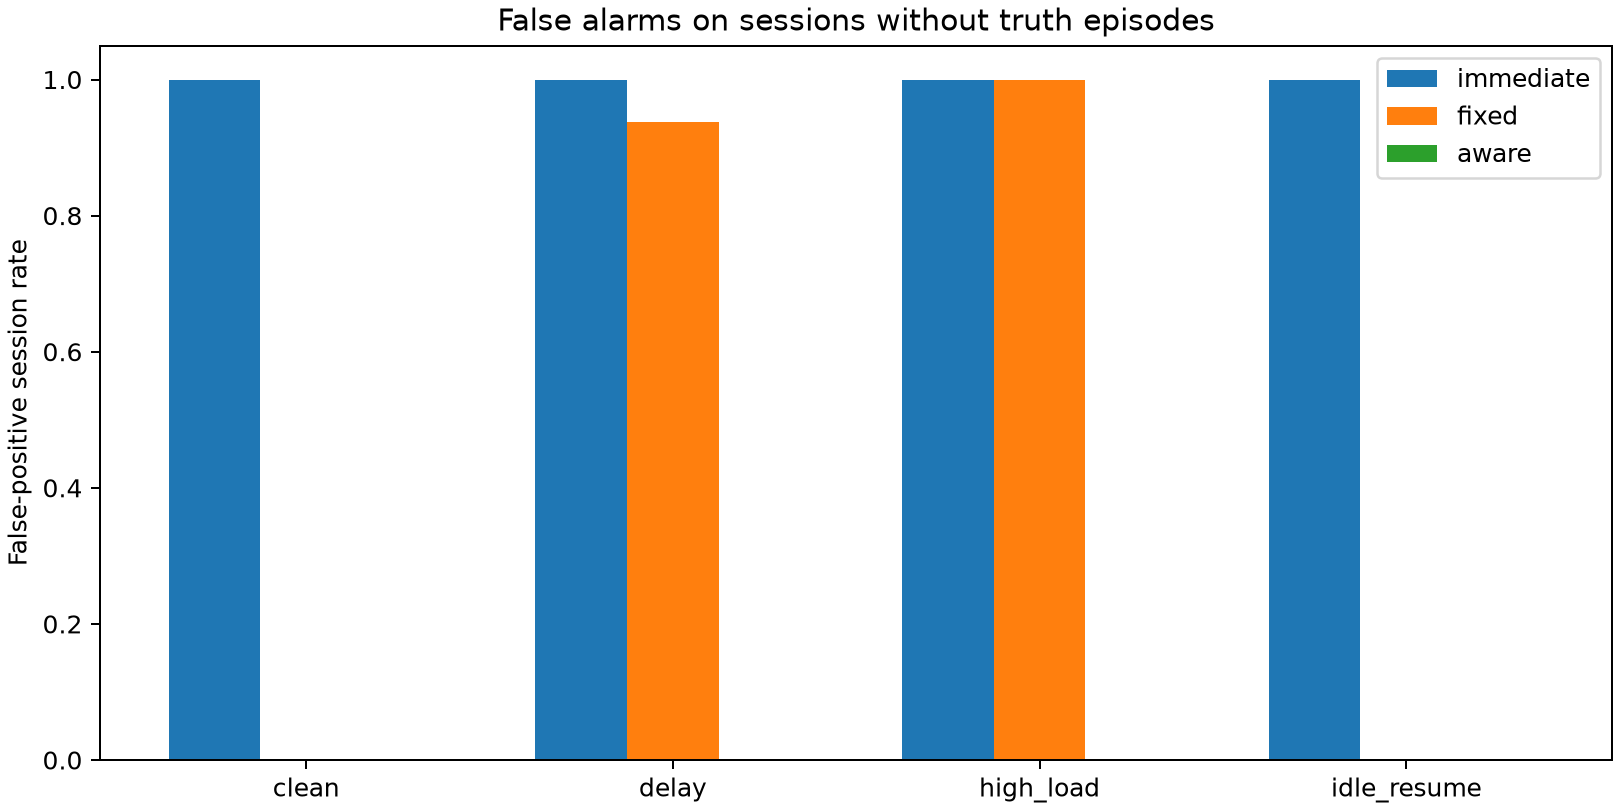
\includegraphics[width=\columnwidth]{../results/final-benchmark/false_positives.png}
\caption{False-positive session rates for the implemented baselines and aware verifier. Results are synthetic and scenario-specific.}
\label{fig:fp}
\end{figure}

Clean, request-failure, reordered-observation, idle/resume and local-cell controls also produce no aware false alarms.

\subsection{Recovery Effectiveness}
Table~\ref{tab:recovery} compares paired recovery-off/on runs. Each row contains 720 probes. For QoS completion failures, all 167 recovery jobs converge, but 148 probes still fail because some probes precede successful intervention. Therefore 100\% job success does not mean that every downstream probe succeeds.
\begin{table}[t]
\caption{Recovery Results Across 40 Paired Seeds}
\label{tab:recovery}\centering\small
\begin{tabular}{lrrr}
\toprule Scenario & Failed probes & Failed probes & Successful\\
 & off & on & jobs\\\midrule
Setup completion & 334 & 0 & 167/167\\
QoS completion & 334 & 148 & 167/167\\
Release completion & 167 & 41 & 167/167\\
Queued high load & 267 & 21 & 154/154\\
Observation outage & 334 & 334 & 15/167\\
Adapter unavailable & 334 & 334 & 0/167\\\bottomrule
\end{tabular}
\end{table}

QoS mismatch exposure falls from 15,698 to 6,192 session-ms, a 60.56\% reduction. Failed probes fall by 55.69\%. These totals aggregate 40 seeds rather than describe one trace. Setup recovery can remove orphan resources and make consistency probes pass without re-establishing a desired session. Observation outages leave little intervention time before later operations and trigger pending/version refusals. An unavailable adapter produces no successful reconciliation.

\subsection{Timing Sensitivity and Software Checks}
The held-out suite varies polling over 5, 15, 30 and 90 ms and grace over 0, 12 and 24 ms for QoS completion failure, benign delay and observation reordering. With 12 ms grace, QoS completion failure yields 77 detected episodes and zero misses at each polling interval. Mean detection delays are 15.69, 21.61, 23.48 and 23.51 ms respectively. Event-triggered snapshots remain enabled, so polling interval is not total observation latency.

The implementation passes 48 behavioral and integration tests, including dashboard tests. Recorded core line coverage is 98.9\%. Code and type checks pass. A review fixed source-hash collection to resolve from the package location, enabling experiment provenance when launched from a different working directory. A Windows launcher invokes the existing environment directly. These software checks support reproducibility, not 3GPP certification.

\section{Limitations and Threats to Validity}
The simulator abstracts resource transactions and does not encode full NAS, NGAP, QoS-flow/DRB mapping, independent N4 behavior or handover signaling. RRC access controls are limited. Commit policy, timeouts, delay distributions and Core authority are declared experimental assumptions.

Complete snapshots, reliable identities, monotonic sequences and a common clock simplify observation. Real deployments require instrumented adapters, authenticated telemetry, identity correlation and conservative clock-skew bounds. Packet traces alone may not reveal internal committed state. The shared oracle predicates limit independent validation of semantic correctness.

Six sessions per run and a finite horizon do not establish scalability. Snapshot storage is $O(S)$ for $S$ sessions, but the current checker scans candidate keys inside its session loop and can require $O(S^2)$ work per tick. An indexed candidate structure and measured larger workloads are future work. Local execution time is not production monitoring latency.

Consistency probes do not measure throughput or calls. Recovery can restore agreement by deactivating resources; failed requests can harm availability without desynchronization. The baselines are task ablations, not replicas of the cited AI system.

\section{Conclusion}
This project implements and evaluates an explainable verifier for a scoped RAN--Core context model. Fresh and temporally aligned observations, procedure guards and persistence distinguish modeled stable contradictions from valid temporary disagreement. The 2,640-run evaluation demonstrates zero aware false alarms in selected benign controls and lower mismatch exposure when bounded recovery is available. The next step is independent validation on instrumented RAN/Core software with user-plane demand, clock skew, concurrent operations and genuine mobility procedures.

\section*{Reproducibility}
The package includes code, tests, a formal model and locked dependencies. Main results are in \texttt{results/final-benchmark/} (seeds 1--40); held-out results are in \texttt{results/sensitivity.csv}. The Windows launcher \texttt{run.ps1} accepts \texttt{app}, \texttt{test}, \texttt{benchmark} or \texttt{sensitivity}. Paths are relative to the project root.

\begin{thebibliography}{9}
\bibitem{cho} Y.-J. Cho et al., ``A Framework for AI-Based Large-Scale Time-Series Anomaly Detection in 5G Core Networks,'' in \textit{Proc. IEEE ICTC}, 2025, doi: 10.1109/ICTC66702.2025.11388910.
\bibitem{procedures} 3GPP, ``Procedures for the 5G System (5GS); Stage 2,'' TS 23.502, V16.18.0, secs. 4.3.2--4.3.4.
\bibitem{ngap} 3GPP, ``NG Application Protocol (NGAP),'' TS 38.413, V16.5.0, secs. 8.2.1--8.2.3.
\bibitem{transport} 3GPP, ``NG signalling transport,'' TS 38.412, V16.0.0, 2020, secs. 4.1 and 7.
\bibitem{consistency} J. Sid-Otmane, S. Imadali, F. Martelli, and M. Shapiro, ``Data Consistency in the 5G Specification,'' in \textit{Proc. ICIN}, 2020, pp. 110--117, doi: 10.1109/ICIN48450.2020.9059408.
\bibitem{ran} 3GPP, ``NR; NR and NG-RAN Overall Description; Stage 2,'' TS 38.300, V16.2.0, 2020.
\bibitem{simpy} SimPy, ``Discrete-event simulation framework,'' [Online]. Available: \url{https://simpy.readthedocs.io/}.
\bibitem{streamlit} Streamlit, ``Documentation,'' [Online]. Available: \url{https://docs.streamlit.io/}.
\end{thebibliography}
\end{document}
